\documentclass[12pt, titlepage]{article}

\usepackage{cite}
\usepackage{booktabs}
\usepackage{tabularx}
\usepackage{hyperref}
\usepackage{amssymb}
\usepackage{amstext}
\usepackage{amsthm}
\usepackage{amsmath}
\usepackage{enumerate}
\usepackage{fancyhdr}
\usepackage[margin=1in]{geometry}
\usepackage{graphicx}
\usepackage{extarrows}
\usepackage{setspace}
\usepackage{adjustbox}
\usepackage{hyperref}


\hypersetup{
    colorlinks,
    citecolor=black,
    filecolor=black,
    linkcolor=red,
    urlcolor=blue
}
\usepackage[round]{natbib}

\title{SE 3XA3: Test Report\\SocialPy}

\author{
	Team 1, SocialPy
		\\ Anando Zaman, zamana11
        \\ Graeme Woods, woodsg1
        \\ Yuvraj Randhawa, randhawy
        \\ Due April 12, 2021
        \\ Tag TR-Rev.1
}

\date{\today}

\begin{document}

\maketitle

\pagenumbering{roman}
\tableofcontents
\listoftables
\listoffigures

\newpage
\begin{table}[!hbp]
    \caption{Revision History} \label{RevisionHistory}
    \begin{tabularx}{\textwidth}{llX}
        \toprule
            \textbf{Date} & \textbf{Developer(s)} & \textbf{Change}\\
        \midrule
            March 25, 2021 & Anando Zaman & Copy template\\
        \bottomrule
    \end{tabularx}
\end{table}
\newpage

\pagenumbering{arabic}

This document contains all the results of the planned tests that were defined in the test plan.

\section{Functional Requirements Evaluation}
\begin{enumerate}

\item{\textbf{FR-ST-2}}

Initial State: Existing account with same email exists in database.
					
Input: Email address and password
					
Expected Output: Returns "Login Successful!" message and updates $self.user$

Actual Output: Returns "Login Successful!" message and updates $self.user$
					
Result: Pass
\end{enumerate}

\paragraph{Register new users}
\begin{enumerate}

\item{\textbf{FR-ST-3}}

Initial State: Existing account with same email does NOT already exist in database.
					
Input: Email address and password
					
Expected Output: Returns "Account profile successfully made!" message and updates $self.user$ object

Actual Output: Returns "Account profile successfully made!" message and updates $self.user$ object
					
Result: Pass
\end{enumerate}

\paragraph{Reset account password}
\begin{enumerate}

\item{\textbf{FR-ST-6}}

Type: Functional, Manual.
					
Initial State: Existing account with same email already exists in the database
					
Input: Email address
					
Expected Output: Firebase sends a email to reset the users' password in which they will enter their new password.

Actual Output: Firebase sends a email to reset the users' password in which they will enter their new password.

Result: Pass

\end{enumerate}

\subsubsection{Post subsystem tests}
		
\paragraph{Query all posts data}

\begin{enumerate}

\item{\textbf{FR-ST-1}}

Type: Functional, Dynamic, Unit, Automated.
					
Initial State: Firebase contains predefined JSON structure already completed
					
Input: "POST VIEW ALL" string
					
Expected Output: Returns string containing all the posts from the database.

Actual Output: Returns string containing all the posts from the database.
					
Result: Pass
\end{enumerate}

\paragraph{Query posts by username}	
\begin{enumerate}
\item{\textbf{FR-ST-4}}

Type: Functional, Dynamic, Unit, Automated.
					
Initial State: Database contains atleast one post and atleast one username.
					
Input: "POST VIEW username"
					
Output: Returns a string containing all the posts for a given user along with the timestamp of when post was created.


Actual Output: Returns a string containing all the posts for a given user along with the timestamp of when post was created.
					
Result: Pass
\end{enumerate}

\paragraph{Delete post}	
\begin{enumerate}
\item{\textbf{FR-ST-5}}

Type: Functional, Manual.
					
Initial State: Database contains atleast one post for the current logged in user with the matching post\_id.
					
Input: "POST DELETE post\_id"
					
Output: Returns a string that says ``post deleted".


Actual Output: Returns a string that says ``post deleted".
					
Result: Pass
\end{enumerate}

\paragraph{Add post}	
\begin{enumerate}
\item{\textbf{FR-ST-8}}

Type: Functional, Dynamic, Unit, Automated.
					
Initial State: Database contains a valid "posts" branch for the post to be added to.
					
Input: "POST ADD post\_id"
					
Output: Returns a message informing the user that "post content has been added". The database reflects the changes made in the users' post branch.


Actual Output: Returns a message informing the user that "post content has been added". The database reflects the changes made in the users' post branch.
					
Result: Pass
\end{enumerate}

\paragraph{Edit post}	
\begin{enumerate}
\item{\textbf{FR-ST-9}}

Type: Functional, Manual.
					
Initial State: Database contains a valid "posts" branch for the post to be added to.
					
Input: "POST EDIT post\_id" followed by the user entering the modified post.
					
Output: Returns "post has been updated" message and post content becomes updated in the database.


Actual Output: Returns "post has been updated" message and post content becomes updated in the database.
					
Result: Pass
\end{enumerate}

\paragraph{Help commands}	
\begin{enumerate}
\item{\textbf{FR-ST-10}}

Type: Functional, Manual
					
Initial State: User is logged into the system.
					
Input: User inputs "Help"
					
Output: Returns a message with all the commands available.

Actual Output: Returns a message with all the commands available.
					
Result: Pass
\end{enumerate}

\subsubsection{Profile subsystem tests}
		
\paragraph{Query Profile}

\begin{enumerate}

\item{\textbf{FR-ST-11}}

Type: Functional, Dynamic, Unit, Automated.
					
Initial State: The user profile exists in the database.
					
Input: "PROFILE VIEW ALL" string
					
Output: Returns string containing all the profile information(location, name, followers) from the database.


Actual Output: Returns string containing all the profile information(location, name, followers) from the database.
					
Result: Pass
\end{enumerate}

\paragraph{Edit Profile Location}

\begin{enumerate}

\item{\textbf{FR-ST-12}}

Type: Functional, Dynamic, Unit, Automated.
					
Initial State: The user profile exists in the database.
					
Input: "PROFILE EDIT\_LOCATION location\_name" string
					
Output: Returns a "Successfully updated location" message. The database reflects the changes made. 

Actual Output: Returns a "Successfully updated location" message. The database reflects the changes made. 
					
Result: Pass
\end{enumerate}

\paragraph{Edit Profile Name}

\begin{enumerate}

\item{\textbf{FR-ST-13}}

Type: Functional, Dynamic, Unit, Automated.
					
Initial State: The user profile exists in the database.
					
Input: "PROFILE EDIT\_NAME name" string
					
Output: Returns a ``Name has been set to `inputted name'" message. The database reflects the changes made. 


Actual Output: Returns a ``Name has been set to `inputted name'" message. The database reflects the changes made. 
					
Result: Pass
\end{enumerate}

\paragraph{Delete Account}

\begin{enumerate}

\item{\textbf{FR-ST-14}}

Type: Functional, Dynamic, Manual.
					
Initial State: The user profile exists in the database.
					
Input: "PROFILE DELETE ACCOUNT" string
					
Output: Returns a "Succussfully removed account!" message. Removes user profile and posts associated with the user from the database.


Actual Output: Returns a "Succussfully removed account!" message. Removes user profile and posts associated with the user from the database.
					
Result: Pass
\end{enumerate}

\paragraph{Delete Follower}

\begin{enumerate}

\item{\textbf{FR-ST-15}}

Type: Functional, Dynamic, Unit, Automated.
					
Initial State: The follower to be deleted exists in the users following list. The user is also logged in.
					
Input: "PROFILE FOLLOWINGS\_DELETE username" string
					
Output: Returns a "`username' was successfully removed from your followers list" message. Removes user from following list in the database.


Actual Output: Returns a "`username' was successfully removed from your followers list" message. Removes user from following list in the database.
					
Result: Pass
\end{enumerate}

\paragraph{Add Follower}

\begin{enumerate}

\item{\textbf{FR-ST-7}}

Type: Functional, Dynamic, Unit, Automated.
					
Initial State: The follower to be added does NOT already exist in the users following list. The user is also logged in.
					
Input: "PROFILE FOLLOWINGS\_ADD username" string
					
Expected Output: Returns a "[username] was successfully added to your followings list!" message. Adds the username to follower list in the database.

Actual Output: Returns a "[username] was successfully added to your followings list!" message. Adds the username to follower list in the database.
					
Result: Pass
\end{enumerate}

\paragraph{View Followers}

\begin{enumerate}

\item{\textbf{FR-ST-16}}

Type: Functional, Dynamic, Unit, Automated.
					
Initial State: The user is logged in. The username to view followers is valid/exists on database.
					
Input: "PROFILE FOLLOWERS\_VIEW username" string
					
Output: Returns a string containing all the followers for a given username separate by new-line characters.


Actual Output: Returns a string containing all the followers for a given username separate by new-line characters.
					
Result: Pass
\end{enumerate}

\subsection{Tests for Nonfunctional Requirements}

\subsubsection{Look and Feel Requirements}
		
\paragraph{Appearance Requirements}

\begin{enumerate}

\item{NFR-LF-1\\}

Type: Manual, Dynamic, Checklist
					
Initial State: SocialPy is active and running
					
Input/Condition: Set of all SocialPy commands entered
					
Expected Output: Outputs the results of the commands in the terminal as text format.
					
Actual Output: Outputs the results of the commands in the terminal as text format.
					
Result: Pass

\end{enumerate}

\paragraph{Style Requirements}

\begin{enumerate}

\item{NFR-LF-2\\}

Type: Manual, Usability Survey

Outcome: All four users stated that the text and menus were easy to comprehend and self-explanatory.			
					
Result: Pass

\item{NFR-LF-3\\}

Type: Manual, Usability Survey

Outcome: All four users stated that	the color scheme was good since it is a terminal program, so they had no complaints about the black and white color scheme.		
					
Result: Pass
\end{enumerate}

\subsubsection{Usability and Humanity Requirements}
\paragraph{Ease of use Requirements}
\begin{enumerate}

\item{NFR-UH-4\\}

Type: Manual, Usability Survey
					
Outcome: The user has agreed to our terms when signing up that they must be 13 or over to access the service.
					
Result: Pass

\item{NFR-UH-5\\}

Type: Manual, Usability Survey
					
Outcome: The average user was able to navigate between tasks in around 5 seconds.
					
Result: Pass

\paragraph{Personalization and Internationalization Requirements}
\item{NFR-UH-6\\}

Type: Manual, checklist

Initial State: SocialPy is waiting for input
					
Input/Condition: English words and Russian words.
					
Expected Output/Result: Outputs "Sorry, your command is invalid. Please type 'help' if you need to view the list of commands!" if in Russian input. Outputs no error message if valid command in English.
		
Actual Output: "Sorry, your command is invalid. Please type 'help' if you need to view the list of commands!" for russian words.
					
Result: Pass

\end{enumerate}
\newpage
\subsubsection{Performance Requirements}
\paragraph{Speed Requirements}
\begin{enumerate}
    \item{NFR-PR-7\\}
    
    Type: Automated, Dynamic, UnitTest
    
    Initial State: Data to query exists in DB
    					
    Input/Condition: set of data branches to query
    					
    Expected: Outputs the time required to query each branch
    					
    Actual Output: Outputs the time required to query each branch
    					
    Result: Pass
    
    \item{NFR-PR-8\\}
    
    Type: Automated, Dynamic, UnitTest
    
    Initial State: Waiting for user credentials. User account already exists in the DB.
    					
    Input/Condition: email and password credentials.
    					
    Expected Output/Result: Outputs the time required to authenticate, boolean value indicating if less than 4 seconds.
    					
    Actual Output: Outputted 1.354 seconds 
    					
    Result: Pass

\end{enumerate}

\paragraph{Precision or Accuracy Requirements}
\begin{enumerate}
    \item{NFR-PR-9\\}
    
    Type: Automated, Dynamic, UnitTest
    
    Initial State: Atleast one post exists in DB for the given user.
    					
    Input/Condition: Query post for the given user.
    					
    Expected Output/Result: Outputs the the timestamp data.
    					
    Actual Output: Outputs the the timestamp data.
    					
    Result: Pass
    
\item{NFR-PR-10\\}
    
    Type: Automated, Dynamic, UnitTest
    
    Initial State: The user is logged in prior to posting.
    					
    Input/Condition: Post string content
    					
    Expected Output/Result: 'Post "{postContent}" added'
    					
    Actual Output: 'Post "{postContent}" added'
    					
    Result: Pass

\end{enumerate}

\paragraph{Reliability and Availability Requirements}
\begin{enumerate}
    \item{NFR-PR-11\\}
    
    Type: Manual, Dynamic
    
    Expected Output: System will have 99\% uptime.
    
    Actual Output: The firebase cloud console shows statistics with currently zero downtime, thus satisfies the availability requirement thus far.
    					
    Result: Pass
 \end{enumerate}   
 
 \paragraph{Scalability or Extensibility Requirements}
\begin{enumerate}
    \item{NFR-PR-12\\}
    
    Type: Manual, Dynamic
    
    Initial State: No commands being made
    
    Input: Post(add,view) commands being made by 5 users at the same time.
    
    Expected Output: System returns the response at the time of output without having duplicate posts of the same post\_id.
    
    Actual Output: System returns the response at the time of output without having duplicate posts of the same post\_id. Each postID is unique, thus no duplication on posts.
    					
    Result: Pass
    
    \item{NFR-PR-13\\}
    
    Type: Manual, Dynamic
    
    Initial State: No commands being made
    
    Input: Execute 20 Post(add,view) commands
    
    Expected Output: System returns the success response message of each post.
    
    Actual Output: System returns the success response message of each post.
    
    Result: Pass
    

 \end{enumerate}  

\subsubsection{Operational and Environmental Requirements}
\paragraph{Expected Physical Environment}
\begin{enumerate}
    \item{NFR-OE-14\\}
    
    Type: Manual, Dynamic
    
    Outcome: The team was able to run the program using Python 3.7 without any errors.
    
    Result: Pass
    
    \item{NFR-OE-15\\}
    
    Type: Manual, Dynamic
    
    Outcome: the team disabled the internet connection and received an error but when the connection was restored SocialPy functioned as usual.
    					
    Result: Pass
    

 \end{enumerate} 
 
 \paragraph{Requirements for interfacing with Adjacent Systems}
\begin{enumerate}
    \item{NFR-OE-16\\}
    
    Type: Automatic, Dynamic, Unittest
    
    Initial State: No commands being made, SocialPy waiting for command. username to be queried already exists in Firebase.
    
    Input: "POST VIEW username" command
    
    Expected Output: System returns the post
    
    Actual Output: System returns the post
    					
    Result: Pass
    

 \end{enumerate} 
 
  \paragraph{Installability Requirements}
\begin{enumerate}
    \item{NFR-OE-17/18 \\}
    
    Type: Manual, Dynamic
    Initial state: Program does not exist on the users computer.
    
    Input: "git clone gitlab\_project" and double click $main.py$
    
    Expected Output: Project successfully cloned and SocialPy login screen appears.
    
    Actual Output: Project successfully cloned and SocialPy login screen appears.
    					
    Result: Pass
    

 \end{enumerate} 
 
   \paragraph{Installability Requirements}
\begin{enumerate}
    \item{NFR-OE-19 \\}
    
    Type: Manual, Dynamic
    
    Initial state: Program cloned on atleast 3 computers.
    
    Input: double click $main.py$
    
    Expected Output: SocialPy login screen appears.
    
    Actual Output: SocialPy login screen appears.
    					
    Result: Pass
    

 \end{enumerate} 
 
    \paragraph{Release Requirements}
\begin{enumerate}
    \item{NFR-OE-20 \\}
    
    Type: Manual, static, code inspection
    Initial state: Program deployed to users in production
    Input: Users provide feedback and feature requests
    Expected Output: Development team maintains feedback via a Gitlab issue tracker.
    
    Actual Output:
    					
    Result:
    

 \end{enumerate} 

\subsubsection{Maintainability and Support Requirements}
\paragraph{Maintenance Requirements}
\begin{enumerate}
    \item{NFR-MS-21\\}
    
    Type: Manual, Static
    
    Initial state: N/A
    
    Input: N/A
    
    Expected Output: The code is documented accurately with comments

    Actual Output: The code is documented accurately with comments
    					
    Result: Pass
    
    \item{NFR-MS-22\\}
    Type: Manual, Static
    
    Outcome: Our documentation has been sufficiently reviewed by the group and is easily understandable. 
    					
    Result: Pass
    
    \item{NFR-MS-23\\}
    Type: Manual, Static
    
    Initial state: Doxygen documents have not been created
    
    Input: Generate Doxygen documents (HTML and pdf)
    
    Expected Output: Doxygen documents are generated successfully
    
    Actual Output: Doxygen documents are generated successfully
    					
    Result: Pass
    
 \end{enumerate} 
 
 \paragraph{Supportability Requirements}
\begin{enumerate}
    \item{NFR-MS-24\\}
    
    Type: Manual, Dynamic
    
    Initial state: SocialPy is actively running
    
    Input: User would like to view the commands that they are able to execute so the run the $help$ command.
    
    Expected Output: List of all the commands is displayed for the user
    
    Actual Output:  List of all the commands is displayed for the user
    					
    Result: Pass

 \end{enumerate} 
 
 \paragraph{Longevity Requirements}
\begin{enumerate}
    \item{NFR-MS-26\\}
    
    Type: Manual, Static
    
    Outcome: The code has been sufficiently divided into its respective modules and classes to allow for longevity.
    					
    Result: Pass
    
    
 \end{enumerate} 
 
\subsubsection{Security Requirements}
 \paragraph{Access and Confidentiality Requirements}
\begin{enumerate}
    \item{NFR-SR-28\\}
    
    Type: Manual, static, code inspection
    
    Output: No data inconsistencies or exposed API endpoints found. No confidential data is stored locally, and all communication is done through secure HTTP API requests.
    
    Result: Pass
    
    \item{NFR-SR-29\\}
    Type: Manual, Dynamic, 
    
    Initial state: Database does not have users' email already registered.
    
    Input: User tries to login using a set of invalid credentials and symbols
    
    Expected Output: System outputs "invalid credentials" message and prevents them from proceeding any further.
    
    Actual Output: System outputs "invalid credentials" message and prevents them from proceeding any further.
    					
    Result: Pass
    
 \end{enumerate} 
 
 \paragraph{Integrity Requirements}
\begin{enumerate}
    \item{NFR-SR-30\\}
    
    Type: Manual, Dynamic.
    
    Initial state: Database contains at least one user account
    
    Input: Email and password credentials for login. "POST ADD content" command afterwards.
    
    Expected Output: Success message for logging in and adding a post. Failure message if unable to login due to invalid credentials.
    
    Actual Output: Success message for logging in and adding a post. Failure message if unable to login due to invalid credentials.
    					
    Result: Pass
 \end{enumerate} 
 
 \begin{enumerate}
    \item{NFR-SR-31\\}
    
    Type: Automated, Dynamic.
    
    Initial state: Zero timeouts and attempts
    
    Input: Email and password credentials for login.
    
    Expected Output: "Too many failed login attempts. Please try again after 10 seconds..."
    
    Actual Output: "Too many failed login attempts. Please try again after 10 seconds..."
    					
    Result: Pass
 \end{enumerate} 

\newpage
\section{Comparison to Existing Implementation}
When comparing the testing of the original open-source project and the current re-developed project (SocialPy), there are some notable changes. However, the architecture remains the same and thus the testing is quite similar. The original implementation had unit tests for all of the common modules to test for boundary and edge cases. The modules that were tested in the original implementation include AddPost, ViewPost, and CommandParser. Our re-implementation had several other unit tests due to additional features that were added to the program such as authentication, deletion of posts, view/modification of following/followers along with profile View/Edit functionality. Each of these were tested using a combination of unit tests and manual tests whereas the original implementation used only unit tests. Our implementation includes data persistence via a NoSQL database whereas the original implementation has no way to save application data. Without much setup (other than authentication), our tests can login and run tests on existing users and posts that are already in the database. The open-source application had to create "dummy" posts and users before running the tests since it had no data persistence. In summary, the structure of the tests was the same as each of the unit tests were put in the unit tests folder and were tested for boundary and edge cases. The differences lie on the number of tests due to extended functionality along with slight differences due to data querying as the original implementation did not have a database to persist the data.

\section{Unit Testing}
Unit tests were performed using the Python Unittest framework. Statement coverage was analyzed using the same testing library. Specific code for the unit tests can be found in 

\href{https://gitlab.cas.mcmaster.ca/zamana11/se3xa3-project/-/tree/master/src/Social\%20Media\%20App/UnitTests}{https://gitlab.cas.mcmaster.ca/zamana11/se3xa3-project/-/tree/master/src/Social\%20Media\%20App/UnitTests} 


\section{Changes Due to Testing}
There was no changes to the code upon testing as the actual outcomes matched our desired targets. All functional and non-functional requirements were validated and showed no signs of inconsistencies. Thus, no changes were made to the source code upon analyzing the results of the tests.

\section{Automated Testing}
Automated testing was used for a large majority of the modules and functional requirements using the Python Unittest framework. However, there was also some parts that were infeasible for automated testing aswell due to requiring several user commands with the UI which could not be simulated easily. For these specific instances, manual testing was done verify these requirements.
		
\section{Trace to Requirements}
\noindent Test IDs correspond to the tests found in this document. Requirement IDs correspond to the requirements found in the SRS. \\

\begin{table}[htbp]
    \centering
    \caption{Traceability Matrix: Functional Requirement}
    \begin{adjustbox}{max width=0.7\paperwidth}
    \begin{tabular}{l|ccccccccccccccccc}
        \textbf{Test IDs} & \multicolumn{11}{c}{\textbf{Requirement IDs}}\\
        \hline
        ~ & \textbf{FR1} & \textbf{FR2} & \textbf{FR3} & \textbf{FR4} & \textbf{FR5} & \textbf{FR6} & \textbf{FR7} & \textbf{FR8} & \textbf{FR9} & \textbf{FR10} & \textbf{FR11} & \textbf{FR12} & \textbf{FR13} & \textbf{FR14} & \textbf{FR15} & \textbf{FR15}\\
        \textbf{FR-ST-1}    & X & ~ & ~ & ~ & ~ & ~ & ~ & ~ & ~ & ~ & ~\\
        \textbf{FR-ST-2}  & ~ & X & ~ & ~ & ~ & ~ & ~ & ~ & ~ & ~ & ~\\
        \textbf{FR-ST-3}  & ~ & ~ & X & ~ & ~ & ~ & ~ & ~ & ~ & ~ & ~\\
        \textbf{FR-ST-4}  & ~ & ~ & ~ & X & ~ & ~ & ~ & ~ & ~ & ~ & ~\\
        \textbf{FR-ST-5}  & ~ & ~ & ~ & ~ & X & ~ & ~ & ~ & ~ & ~ & ~\\
        \textbf{FR-ST-6}  & ~ & ~ & ~ & ~ & ~ & X & ~ & ~ & ~ & ~ & ~\\
        \textbf{FR-ST-7}  & ~ & ~ & ~ & ~ & ~ & ~ & X & ~ & ~ & ~ & ~\\
        \textbf{FR-ST-8}  & ~ & ~ & ~ & ~ & ~ & ~ & ~ & X & ~ & ~ & ~\\
        \textbf{FR-ST-9}  & ~ & ~ & ~ & ~ & ~ & ~ & ~ & ~ & X & ~ & ~\\
        \textbf{FR-ST-10}  & ~ & ~ & ~ & ~ & ~ & ~ & ~ & ~ & ~ & X & ~\\
        \textbf{FR-ST-11}  & ~ & ~ & ~ & ~ & ~ & ~ & ~ & ~ & ~ & ~ & X\\
        \textbf{FR-ST-12}  & ~ & ~ & ~ & ~ & ~ & ~ & ~ & ~ & ~ & ~ & ~ & X\\
        \textbf{FR-ST-13}  & ~ & ~ & ~ & ~ & ~ & ~ & ~ & ~ & ~ & ~ & ~ & ~ & X\\
        \textbf{FR-ST-14}  & ~ & ~ & ~ & ~ & ~ & ~ & ~ & ~ & ~ & ~ & ~ & ~ & ~ & X\\
        \textbf{FR-ST-15} & ~ & ~ & ~ & ~ & ~ & ~ & ~ & ~ & ~ & ~ & ~ & ~ & ~ & ~ & X\\
        \textbf{FR-ST-16} & ~ & ~ & ~ & ~ & ~ & ~ & ~ & ~ & ~ & ~ &  ~ & ~ & ~ & ~ & ~ & X\\
    \end{tabular}
    \end{adjustbox}
    \label{Traceability Matrix: Functional Requirement}
\end{table}

\newpage
\begin{table}[htbp]
    \centering
    \caption{Traceability Matrix: Non-functional Requirement}
    \begin{adjustbox}{max width=0.7\paperwidth}
    \begin{tabular}{l|ccccccccccccccccccccccccccccccccccccc}
        \textbf{Test IDs} & \multicolumn{11}{c}{\textbf{Requirement IDs}}\\
        \hline
        ~ & \textbf{NFR1} & \textbf{NFR2} & \textbf{NFR3} & \textbf{NFR4} & \textbf{NFR5} & \textbf{NFR6} & \textbf{NFR7} & \textbf{NFR8} & \textbf{NFR9} & \textbf{NFR10} & \textbf{NFR11} & \textbf{NFR12} & \textbf{NFR13} & \textbf{NFR14} & \textbf{NFR15} & \textbf{NFR16} & \textbf{NFR17} & \textbf{NFR18} & \textbf{NFR19} & \textbf{NFR20} & \textbf{NFR21} & \textbf{NFR22} & \textbf{NFR23} & \textbf{NFR24} & \textbf{NFR25} & \textbf{NFR26} & \textbf{NFR27} & \textbf{NFR28} & \textbf{NFR29} & \textbf{NFR30} & \textbf{NFR31} \\
        \textbf{NFR-LF1}    & X & ~ & ~ & ~ & ~ & ~ & ~ & ~ & ~ & ~ & ~\\
        \textbf{NFR-LF2}  & ~ & X & ~ & ~ & ~ & ~ & ~ & ~ & ~ & ~ & ~\\
        \textbf{NFR-LF3}  & ~ & ~ & X & ~ & ~ & ~ & ~ & ~ & ~ & ~ & ~\\
        \textbf{NFR-UH4}  & ~ & ~ & ~ & X & ~ & ~ & ~ & ~ & ~ & ~ & ~\\
        \textbf{NFR-UH5}  & ~ & ~ & ~ & ~ & X & ~ & ~ & ~ & ~ & ~ & ~\\
        \textbf{NFR-UH6}  & ~ & ~ & ~ & ~ & ~ & X & ~ & ~ & ~ & ~ & ~\\
        \textbf{NFR-PR7}  & ~ & ~ & ~ & ~ & ~ & ~ & X & ~ & ~ & ~ & ~\\
        \textbf{NFR-PR8}  & ~ & ~ & ~ & ~ & ~ & ~ & ~ & X & ~ & ~ & ~\\
        \textbf{NFR-PR9}  & ~ & ~ & ~ & ~ & ~ & ~ & ~ & ~ & X & ~ & ~\\
        \textbf{NFR-PR10}  & ~ & ~ & ~ & ~ & ~ & ~ & ~ & ~ & ~ & X & ~\\
        \textbf{NFR-PR11}  & ~ & ~ & ~ & ~ & ~ & ~ & ~ & ~ & ~ & ~ & X\\
        \textbf{NFR-PR12}  & ~ & ~ & ~ & ~ & ~ & ~ & ~ & ~ & ~ & ~ & ~ & X\\
        \textbf{NFR-PR13}  & ~ & ~ & ~ & ~ & ~ & ~ & ~ & ~ & ~ & ~ & ~ & ~ & X\\
        \textbf{NFR-OE14}  & ~ & ~ & ~ & ~ & ~ & ~ & ~ & ~ & ~ & ~ & ~ & ~ & ~ & X\\
        \textbf{NFR-OE15} & ~ & ~ & ~ & ~ & ~ & ~ & ~ & ~ & ~ & ~ & ~ & ~ & ~ & ~ & X\\
        \textbf{NFR-OE16} & ~ & ~ & ~ & ~ & ~ & ~ & ~ & ~ & ~ & ~ &  ~ & ~ & ~ & ~ & ~ & X\\
        \textbf{NFR-OE17/18} & ~ & ~ & ~ & ~ & ~ & ~ & ~ & ~ & ~ & ~ &  ~ & ~ & ~ & ~ & ~ & ~ & ~ X\\
        \textbf{NFR-OE19} & ~ & ~ & ~ & ~ & ~ & ~ & ~ & ~ & ~ & ~ &  ~ & ~ & ~ & ~ & ~ & ~ & ~ & X \\
        \textbf{NFR-OE20} & ~ & ~ & ~ & ~ & ~ & ~ & ~ & ~ & ~ & ~ &  ~ & ~ & ~ & ~ & ~ & ~ & ~ & ~ & X\\
        \textbf{NFR-MS21} & ~ & ~ & ~ & ~ & ~ & ~ & ~ & ~ & ~ & ~ &  ~ & ~ & ~ & ~ & ~ & ~ & ~ & ~ & ~ & X\\
        \textbf{NFR-MS22} & ~ & ~ & ~ & ~ & ~ & ~ & ~ & ~ & ~ & ~ &  ~ & ~ & ~ & ~ & ~ & ~ & ~ & ~ & ~ & ~ & X\\
        \textbf{NFR-MS23} & ~ & ~ & ~ & ~ & ~ & ~ & ~ & ~ & ~ & ~ &  ~ & ~ & ~ & ~ & ~ & ~ & ~ & ~ & ~ & ~ & ~ & X\\
        \textbf{NFR-MS24} & ~ & ~ & ~ & ~ & ~ & ~ & ~ & ~ & ~ & ~ &  ~ & ~ & ~ & ~ & ~ & ~ & ~ & ~ & ~ & ~ & ~ & ~ & X\\
        \textbf{NFR-MS25} & ~ & ~ & ~ & ~ & ~ & ~ & ~ & ~ & ~ & ~ &  ~ & ~ & ~ & ~ & ~ & ~ & ~ & ~ & ~ & ~ & ~ & ~ & ~ & X\\
        \textbf{NFR-MS26} & ~ & ~ & ~ & ~ & ~ & ~ & ~ & ~ & ~ & ~ &  ~ & ~ & ~ & ~ & ~ & & ~ & ~ & ~ & ~ & ~ & ~ & ~ & ~ & X\\
        \textbf{NFR-MS27} & ~ & ~ & ~ & ~ & ~ & ~ & ~ & ~ & ~ & ~ &  ~ & ~ & ~ & ~ & ~ & & ~ & ~ & ~ & ~ & ~ & ~ & ~ & ~ & ~ & X\\
        \textbf{NFR-SR28} & ~ & ~ & ~ & ~ & ~ & ~ & ~ & ~ & ~ & ~ &  ~ & ~ & ~ & ~ & ~ & & ~ & ~ & ~ & ~ & ~ & ~ & ~ & ~ & ~ & ~ & X\\
        \textbf{NFR-SR29} & ~ & ~ & ~ & ~ & ~ & ~ & ~ & ~ & ~ & ~ &  ~ & ~ & ~ & ~ & ~ & & ~ & ~ & ~ & ~ & ~ & ~ & ~ & ~ & ~ & ~ & ~ & X\\
        \textbf{NFR-SR30} & ~ & ~ & ~ & ~ & ~ & ~ & ~ & ~ & ~ & ~ &  ~ & ~ & ~ & ~ & ~ & & ~ & ~ & ~ & ~ & ~ & ~ & ~ & ~ & ~ & ~ & ~ & ~ & X\\
        \textbf{NFR-SR31} & ~ & ~ & ~ & ~ & ~ & ~ & ~ & ~ & ~ & ~ &  ~ & ~ & ~ & ~ & ~ & & ~ & ~ & ~ & ~ & ~ & ~ & ~ & ~ & ~ & ~ & ~ & ~ & ~ & X\\
    \end{tabular}
    \end{adjustbox}
    \label{Traceability Matrix: Non-functional Requirement}
\end{table}

\newpage
\section{Trace to Modules}
All module IDs were taken from the Module Guide Document.
This is found on the next page.
\begin{table}[htbp]
\centering
\begin{tabular}{p{0.2\textwidth} p{0.6\textwidth}}
\toprule
\textbf{Req.} & \textbf{Modules}\\
\midrule
FR-ST-1 & \mref{M16}\\
FR-ST-2& \mref{M15}, \mref{M16}\\
FR-ST-3 & \mref{M15}, \mref{M16}\\
FR-ST-4 & \mref{M4}, \mref{M5}\\
FR-ST-5 & \mref{M4}, \mref{M2}\\
FR-ST-6 & \mref{M15}, \mref{M16}\\
FR-ST-7 & \mref{M11}, \mref{M12}\\
FR-ST-8 & \mref{M2}\\
FR-ST-9 & \mref{M3}, \mref{M4}\\
FR-ST-10 & \mref{M17}\\
FR-ST-11 & \mref{M13}, \mref{M14}\\
FR-ST-12 & \mref{M9}\\
FR-ST-13 & \mref{M10}\\
FR-ST-14 & \mref{M7}\\
FR-ST-15 & \mref{M8}\\
FR-ST-16 & \mref{M11}, \mref{M12}\\
NFR-LF-1 & \mref{M18}, \mref{M5}, \mref{M12}, \mref{M14}\\
NFR-LF-2 & \mref{M17}\\
NFR-LF-3 & \mref{M18}\\
NFR-UH-5 & \mref{M17}, \mref{M18}\\
NFR-UH-6 & \mref{M18}, \mref{M5}, \mref{M12}, \mref{M14}\\
NFR-PR-7 & \mref{M4}\\
NFR-PR-8 & \mref{M15}\\
NFR-PR-9 & \mref{M4}\\
NFR-PR-10 & \mref{M1}\\
NFR-PR-12 & \mref{M1}, \mref{M2}, \mref{M3}, \mref{M4}, \mref{M5}\\
NFR-OE-16 & \mref{M16}\\
NFR-OE-19 & \mref{M18}\\
NFR-MS-24 & \mref{M17}\\
NFR-MS-26 & \mref{M17}\\
NFR-SR-28 & \mref{M15}\\
NFR-SR-29 & \mref{M15}, \mref{M4}, \mref{M5}\\
NFR-SR-30 & \mref{M15}, \mref{M1}\\
NFR-SR-31 & \mref{M15}\\
\bottomrule
\end{tabular}
\caption{Trace Between Requirements and Modules}
\label{TblRT}
\end{table}

\newpage
\section{Code Coverage Metrics}
Total coverage for the system was 82\% which met our goal of having atleast 80\% code coverage. This is shown on next page.
\begin{figure}[htbp]
\centering
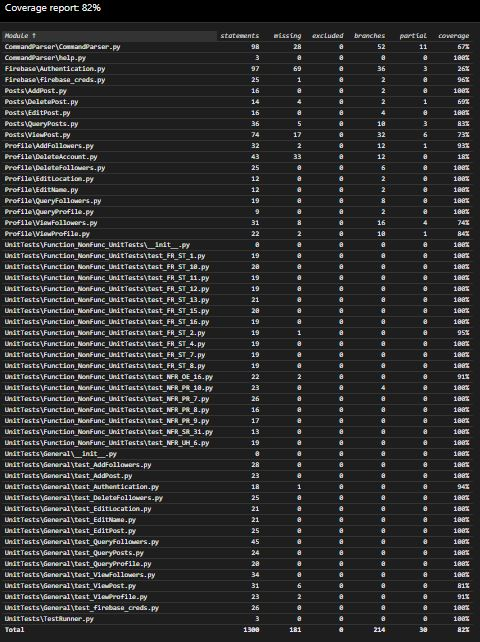
\includegraphics[width=\textwidth]{coverage.JPG}
\caption{Code Coverage Table}
\label{FigUH}
\end{figure}

\bibliographystyle{plainnat}

\bibliography{SRS}

\end{document}